% chapter 4 section 3

\section{磁场}

\subsection{磁场}

\subsubsection{电与磁}

磁的体系与电十分类似,几乎所有磁的概念\footnote{磁场中不存在独立的单极磁荷}都可以在电中找到对应的内容。
\begin{figure}[ht!]
    \centering
    \renewcommand\arraystretch{1.2}
    \begin{tabular}{c|c|c}
        \hline
        &电&磁\\\hline
        基本单位&电荷C&磁荷Wb\\\hline
        场力&电场力(库仑力)&磁场力\\\hline
        场常数&电容率$\varepsilon$(誘電率)&磁导率$\mu$(透磁率)\\\hline
    \end{tabular}
    \caption{电与磁对比}
\end{figure}

因此,磁场的直觉定义即为
\begin{equation*}
    \vec{H}=\frac{\vec{F}}{m}\quad(N/Wb)
\end{equation*}
同样也存在描述磁场走势、大小等信息的磁场线,并具有以下性质。
\begin{itemize}
    \item N极出,S极入
    \item 磁场线密$\iff$磁场强
\end{itemize}
\begin{figure}[ht!]
    \centering
    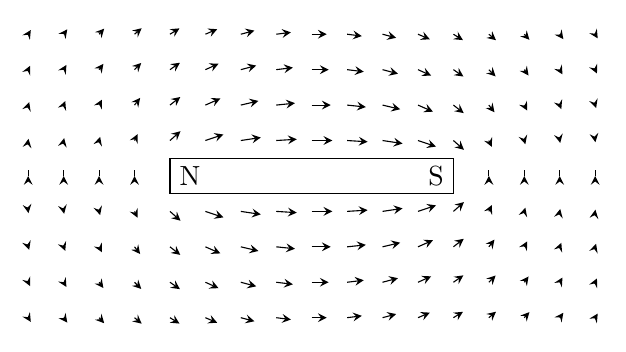
\begin{tikzpicture}[scale=0.45]
        \foreach \x in {-8,...,8} \foreach \y in {-4,...,4} {
            \pgfmathparse{or(
                and(equal(\x,-4),equal(\y,0)),
                and(equal(\x,4),equal(\y,0))
            )}
            \ifnum\pgfmathresult=1
            \else
            \draw[-stealth] (\x,\y) -- ++ (
                {0.3*((\x+4)/sqrt((\x+4)^2+(\y)^2)-(\x-4)/sqrt((\x-4)^2+(\y)^2))},
                {0.3*(\y/sqrt((\x+4)^2+(\y)^2)-\y/sqrt((\x-4)^2+(\y)^2))}
            );
            \fi
        }
        \filldraw[color=black, fill=white] (-4,-0.5) -- node[right] {N} (-4,0.5) -- (4,0.5) -- node[left] {S} (4,-0.5) -- cycle;
    \end{tikzpicture}
    \caption{磁场图示}
\end{figure}

\subsubsection{电生磁}

19世纪初叶,毕奥-萨伐尔定律\footnote{
    Biot-Savart Law
    \begin{equation*}
        \mathbf{B}=\frac{\mu_0}{4\pi}\int\mathbf{J}\times\frac{\mathbf{r}-\mathbf{l}}{|\mathbf{r}-\mathbf{l}|^3}d^3l
    \end{equation*}
}、安培定律\footnote{
    Ampère's circuital law
    \begin{equation*}
        \oint_{\partial S}\mathbf{B}\cdot d\mathbf{l}=\mu_0\int_S\mathbf{J}\cdot d\mathbf{S}
    \end{equation*}
}等揭示了电流的磁作用。下图是三种十分具有代表性的模型,其磁场方向可以由右手螺旋定则判断。
\begin{figure}[ht!]
    \centering
    \begin{minipage}[t]{0.48\textwidth}
        \centering
        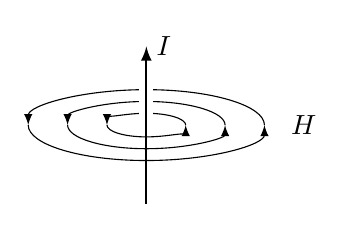
\begin{tikzpicture}
            \foreach \r in {0.5,1,1.5} {
                \draw[-latex] (\r,0) arc (0:180:{\r} and {\r*0.3});
                \draw[-latex] ({-\r},0) arc (-180:0:{\r} and {\r*0.3});
            }
            \draw[color=white, line width=5pt] (0,0) -- (0,1);
            \draw[thick, -latex] (0,-1) -- (0,1) node[right] {$I$};
            \node at (2,0) {$H$};
        \end{tikzpicture}
        \caption{直线电流磁场}
    \end{minipage}
    \begin{minipage}[t]{0.48\textwidth}
        \centering
        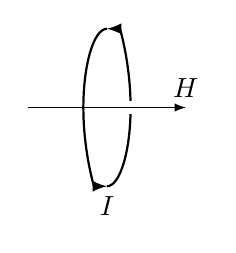
\begin{tikzpicture}
            \draw[thick, -latex] (0,-1) arc (-90:90:0.3 and 1);
            \draw[color=white, line width=5pt] (0,0) -- (1,0);
            \draw[-latex] (-1,0) -- (1,0) node[above] {$H$};
            \draw[thick, -latex] (0,1) arc (90:270:0.3 and 1) node[below] {$I$};
        \end{tikzpicture}
        \caption{环形电流磁场}
    \end{minipage}
    \begin{minipage}{\textwidth}
        \centering
        \begin{tikzpicture}
            \clip (-0.5,-1) rectangle (4,1);
            \draw[thick, midarrow] (0,-1) -- node[left] {$I$} (0,0);
            \draw[thick] (0,0) arc (180:135:0.2 and 0.4);
            \draw[color=white, line width=5pt] (-0.5,0) -- (0.2,0);
            \draw[-latex] (-0.5,0) -- (3.5,0) node[above] {$H$};
            \foreach \n in {0,...,5} {
                \draw[color=white, line width=5pt] ($(0.2+\n*0.4,0)+(135:0.2 and 0.4)$) arc (135:-135:0.2 and 0.4);
                \draw[thick, midarrow] ($(0.2+\n*0.4,0)+(135:0.2 and 0.4)$) arc (135:-135:0.2 and 0.4);
            }
            \draw[color=white, line width=5pt] (2.8,0.2) -- (2.8,-1);
            \draw[thick] ($(2.6,0)+(135:0.2 and 0.4)$) arc (135:0:0.2 and 0.4);
            \draw[thick,midarrow] (2.8,0) -- (2.8,-1);
        \end{tikzpicture}
        \caption{线圈周围磁场}
    \end{minipage}    
\end{figure}
\begin{itembox}[l]{电流产生的磁场}
    \begin{itemize}
        \item 直线电流
        \begin{equation*}
            H=\frac{I}{2\pi r}
        \end{equation*}
        \item 环形电流(中心处)
        \begin{equation*}
            H=\frac{I}{2r}
        \end{equation*}
        \item 线圈
        \begin{equation*}
            H=nI\quad(n:\textrm{线圈匝数})
        \end{equation*}
    \end{itemize}
\end{itembox}

\subsection{安培力}

\subsubsection{平行电流间的力}

\begin{figure}[ht!]
    \centering
    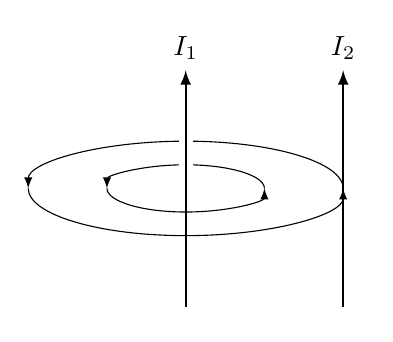
\begin{tikzpicture}
        \draw[-latex] (1,1.5) arc (0:180:1 and 0.3);
        \draw[-latex] (2,1.5) arc (0:180:2 and 0.6);
        \draw[color=white, line width=5pt] (0,0) -- (0,3);
        \draw[thick, -latex] (0,0) -- (0,3) node[above] {$I_1$};
        \draw[-latex] (-1,1.5) arc (180:360:1 and 0.3);
        \draw[-latex] (-2,1.5) arc (180:360:2 and 0.6);
        \draw[thick, -latex] (2,0) -- (2,3) node[above] {$I_2$};
    \end{tikzpicture}
    \caption{平行电流间的力}
\end{figure}
倘若空间中存在两根无限长直导线,分别流过$I_1$与$I_2$大小的电流,那么单位长度的导线上会受到
\begin{equation*}
    f=\frac{\mu I_1I_2}{2\pi r}
\end{equation*}
大小的力。并且当电流同向时表现为吸引力,逆向时表现为排斥力。以$I_1$对$I_2$的视角审视上式则可理解为
\begin{equation*}
    f=\frac{\mu I_1}{2\pi r}I_2=\mu H_1\cdot I_2
\end{equation*}
即$I_2$受到的是来自于$I_1$所产生的磁场导致的力。因此,不难理解通电导线会受到来自于磁场的作用力。

\subsubsection{安培力}

\begin{figure}[ht!]
    \centering
    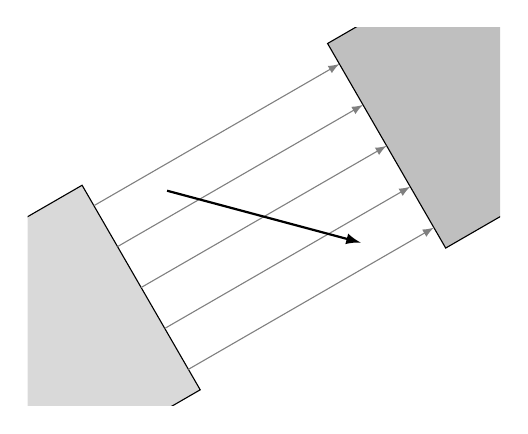
\begin{tikzpicture}[scale=0.6]
        \clip (-5,-4) rectangle (5,4);
        \begin{scope}[rotate=30]
            \filldraw[color=black, fill=gray, fill opacity=0.3] (-8,-2.5) rectangle (-3,2.5);
            \filldraw[color=black, fill=gray, fill opacity=0.5] (3,-2.5) rectangle (8,2.5);
            \foreach \y in {-2,...,2} {
                \draw[color=gray, -latex] (-3,\y) -- (3,\y);
            }
            \draw[thick, -latex] (-1.5,1.5) -- (1.5,-1.5);
            \drawangle{(1,-1)}{(0,0)}{(1,0)};
        \end{scope}
    \end{tikzpicture}
    \caption{安培力}
\end{figure}
上述实验表明将通电导线(电流)置于磁场中,通电导线会受到来自于磁场的力,即\underline{安培力}\footnote{安培力:$\vec{F}=I\vec{l}\times\vec{B}$},大小由$F=\mu HIl$给出。其中$\mu H$的部分也具有实际的物理意义:\underline{磁通量密度}\footnote{可以理解为由环境增强后的磁场。比如向通电线圈内放入铁芯会增强原磁场。},日文为磁束密度,用字母$B$表示。
\begin{itembox}[l]{安培力}
    \begin{equation*}
        F=IBl\sin\theta
    \end{equation*}
    \begin{itemize}
        \item $\theta$:电流方向与磁场方向的夹角
        \item 左手定则
        \begin{itemize}
            \item 磁场穿过手心
            \item 四指与电流同向
            \item 拇指方向为安培力方向
        \end{itemize}
        \item 使用场景:“左力右电”
        \begin{itemize}
            \item 左手定则:电磁力的判断
            \item 右手(螺旋)定则:电磁现象的判断
        \end{itemize}
    \end{itemize}
\end{itembox}

\subsection{洛伦兹力}

\subsubsection{洛伦兹力}

由本章第二节的知识可知,电流是由带电载流子(キャリア)的移动而形成的。因此,重新审视安培力,我们可以认定带电的载流子,比如电子等也会受到磁场的作用。这个力便是洛伦兹力\footnote{洛伦兹力:$\vec{F}=q\vec{v}\times\vec{B}$},日文为ローレンツ力。但使用时需注意\underline{电流方向为正电荷的移动方向}。
\begin{itembox}[l]{洛伦兹力}
    \begin{equation*}
        F=qvB\sin\theta
    \end{equation*}
\end{itembox}

\subsubsection{带电粒子在磁场中的运动}

根据洛伦兹力的性质可知,在粒子运动过程中力与运动方向始终垂直,因此洛伦兹力不做功。结合动能定理可知,粒子运动速度不发生改变,所以作用在其身上的洛伦兹力的大小也将不会改变。基于数学推导可知,当粒子水平入射进入磁场后会做等速圆周运动。
\begin{figure}[ht!]
    \centering
    \begin{tikzpicture}
        \foreach \x in {1,3,5} \foreach \z in {1,3,5} {
            \draw[->, color=gray!80] (\x,-1,\z) -- (\x,0,\z);
        }
        \begin{scope}[xzplane=0]
            \fill[fill=gray!30] (0,0) rectangle (6,6);
            \draw[thick, -latex] (4,3) arc (0:-320:1.5);
        \end{scope}
        \foreach \x in {1,3,5} \foreach \z in {1,3,5} {
            \draw[->, color=gray!80] (\x,0,\z) -- (\x,1.5,\z);
        }
        \fill (4,0,3) circle (2pt) node[below] {$e^-$};
        \draw[thick, -latex] (4,0,3) -- (4,0,2) node[right] {$\vec{v}$};
        \draw[thick, -latex] (4,0,3) -- (2.5,0,3) node[below] {$\vec{F}$};
    \end{tikzpicture}
    \caption{粒子在磁场中的平面运动}
\end{figure}

此时洛伦兹力充当向心力,即
\begin{equation*}
    qvB=m\frac{v^2}{r}
\end{equation*}
则运动半径、周期可求。
\begin{itembox}[l]{粒子在磁场中运动结论}
    \begin{itemize}
        \item 半径:$r=\frac{mv}{qB}$
        \item 周期:$T=\frac{2\pi m}{qB}$
    \end{itemize}
\end{itembox}

当粒子斜向入射进入磁场时,除了垂直于磁场平面上的圆周运动以外,还会在平行于磁场的方向上做匀速直线运动,因此其轨迹将会为圆柱螺线。
\begin{figure}[ht!]
    \centering
    \begin{tikzpicture}
        \foreach \x in {-1,0,1} \foreach \z in {-1,0,1} {
            \draw[->, color=gray!80] (\x,-1,\z) -- (\x,0,\z);
        }
        \begin{scope}[xzplane=0]
            \fill[fill=gray!30] (-1.5,-1.5) rectangle (1.5,1.5);
            \draw[dashed] (0,0) circle (1);
        \end{scope}
        \foreach \x in {-1,0,1} \foreach \z in {-1,0,1} {
            \draw[->, color=gray!80] (\x,0,\z) -- (\x,4,\z);
        }
        \draw[thick, -latex] plot[variable=\t,domain=0:5.5, samples=100,smooth] ({cos((pi*\t) r)},{0.5*\t},{sin((pi*\t) r)});
        \draw[dashed] (1,0,0) -- (1,0,1);
        \draw[thick, -latex] (1,0,0) -- ++ (0,0.5,1);
        \draw[<->] (1.2,0,0) -- node[right] {$v_{z}T$} (1.2,1,0);
    \end{tikzpicture}
    \caption{粒子在磁场中的空间运动}
\end{figure}

此外,体现电磁场共同作用的\underline{霍尔效应}也十分具有代表性。
\begin{figure}[ht!]
    \centering
    \begin{tikzpicture}
        \begin{scope}[yzplane=0] % left
            \filldraw[color=black, dashed, fill=gray, fill opacity=0.3]  (0,0) rectangle (-0.5,3);
            \foreach \z in {0.5,1.5,2.5} {
                \node at (-0.25,\z) {$\ominus$};
            }
        \end{scope}
        \begin{scope}[yzplane=2] % right
            \filldraw[color=black, fill=gray, fill opacity=0.5] (0,0) rectangle (-0.5,3);
            \foreach \z in {0.5,1.5,2.5} {
                \node at (-0.25,\z) {$\oplus$};
            }
        \end{scope}
        \begin{scope}[xzplane=0] % up
            \draw (0,0) rectangle (2,3);
        \end{scope}
        \begin{scope}[xyplane=0] % back
            \draw[dashed] (0,0) rectangle (2,-0.5);
        \end{scope}
        \begin{scope}[xyplane=3] % front
            \draw (0,0) rectangle (2,-0.5);
        \end{scope}
        \draw[thick] (1,-0.25,-1) -- (1,-0.25,0);
        \draw[thick, dashed] (1,-0.25,0) -- (1,-0.25,3);
        \draw[thick, -latex] (1,-0.25,3) -- (1,-0.25,5) node[left] {$I$};
        \draw[thick, -latex] (1,0,1.5) -- (1,1,1.5) node[above] {$B$};
        \node at (3.5,-0.25,5) {$qvB=Eq\implies qB=\frac{V}{vd}$};
    \end{tikzpicture}
    \caption{霍尔效应}
\end{figure}
